\documentclass[10pt,letterpaper]{article}
\usepackage[margin=0.75in]{geometry}
\usepackage{amsmath}
\usepackage{amsfonts}
\usepackage{amssymb}
\usepackage{graphicx}
\usepackage{cancel}
\usepackage{listings}
\usepackage{color}
\usepackage{textcomp}
\definecolor{listinggray}{gray}{0.9}
\definecolor{lbcolor}{rgb}{0.9,0.9,0.9}
\lstset{
	backgroundcolor=\color{lbcolor},
	tabsize=4,
	rulecolor=,
% 	language=Python,
        basicstyle=\scriptsize,
        upquote=true,
        aboveskip={1.5\baselineskip},
        columns=fixed,
        showstringspaces=false,
        extendedchars=true,
        breaklines=true,
        prebreak = \raisebox{0ex}[0ex][0ex]{\ensuremath{\hookleftarrow}},
        frame=single,
        showtabs=false,
        showspaces=false,
        showstringspaces=false,
        identifierstyle=\ttfamily,
        keywordstyle=\color[rgb]{0,0,1},
        commentstyle=\color[rgb]{0.133,0.545,0.133},
        stringstyle=\color[rgb]{0.627,0.126,0.941},
}

\def\mbf{\mathbf}
\def\mbb{\mathbb}

\providecommand{\abs}[1]{\left\lvert#1\right\rvert}
\providecommand{\norm}[1]{\left\lVert#1\right\rVert}
\def\d{\mathrm{d}}
\def\e{\mathrm{e}}

\def\y{\mathbf{y}}
\def\f{\mathbf{f}}
\def\g{\mathbf{g}}
\def\b{\mathbf{b}}

\title{Numerical Treatment of Differential Equations: Homework 5}
\author{Truman Ellis}

\begin{document}
\section*{Problem 3}
The attached code solves the problem
\[
a(x,y)u(x,y)-\mathrm{div}(d(x,y)\mathrm{grad}((u(x,y))))=f(x,y)
\]
for $0\le x\le L_x$, $0\le y\le L_y$ where $u=g(x,y)$ on the boundary.

I chose a fairly difficult problem to stress-test the code, choosing
\begin{align*}
a(x,y)&=\cos(\pi x)\cos(\pi y)\\
d(x,y)&=(x+1)^2(y+1)^2\\
f(x,y)&=\cos(\pi x)\cos(\pi y)\sin(2\pi x^3)\sin(3\pi y^2)\\
&-[2(x+1)(y+1)^2(6\pi x^2\cos(2\pi x^3)\sin(3\pi y^2))\\
&+2(x+1)^2(y+1)(6\pi y\sin(2\pi x^3)\cos(3\pi y^2))\\
&+(x+1)^2(y+1)^2\{-36\pi^2 x^4\sin(2*\pi x^3)\sin(3\pi y^2)\\
&+12\pi x\cos(2\pi x^3)\sin(3\pi y^2)\\
&-36\pi^2 y^2\sin(2\pi x^3)\sin(3\pi y^2)\\
&+6\pi\sin(2\pi x^3)\cos(3\pi y^2)\}]
\end{align*}
with $g(x,y)=0$,
which has exact solution
\[
u(x,y)=\sin(2\pi x^3)\sin(3\pi y^2)\,.
\]
This problem was chosen because it has several Fourier modes in addition to
polynomial growth. If the finite difference solver converges for this problem,
we will know that it was not a coincidence, and that all aspects of the code are
working correctly together.

In Figure \ref{fig:FD} we plot the finite difference solution and in Figure
\ref{fig:Exact} we plot the exact solution.
Finally, in Figure \ref{fig:c} we plot the convergence for this problem.
We do, in fact, get the second order convergence that we were expecting. Thus it
appears that everything is implemented correctly.

\begin{figure}[h]
\begin{center}
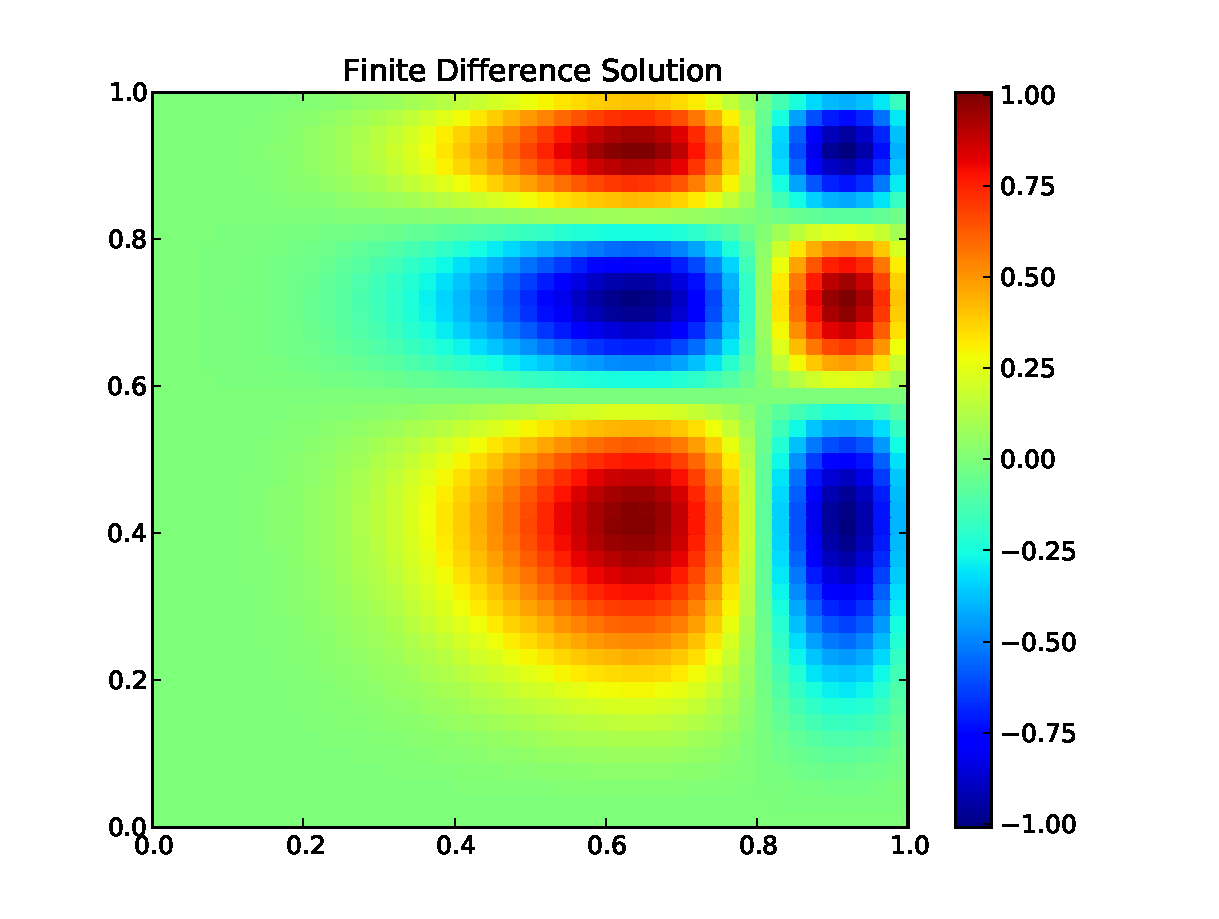
\includegraphics[width=5in,keepaspectratio]{FD.pdf}
\end{center}
\caption{Finite difference solution}
\label{fig:FD}
\end{figure}

\begin{figure}[h]
\begin{center}
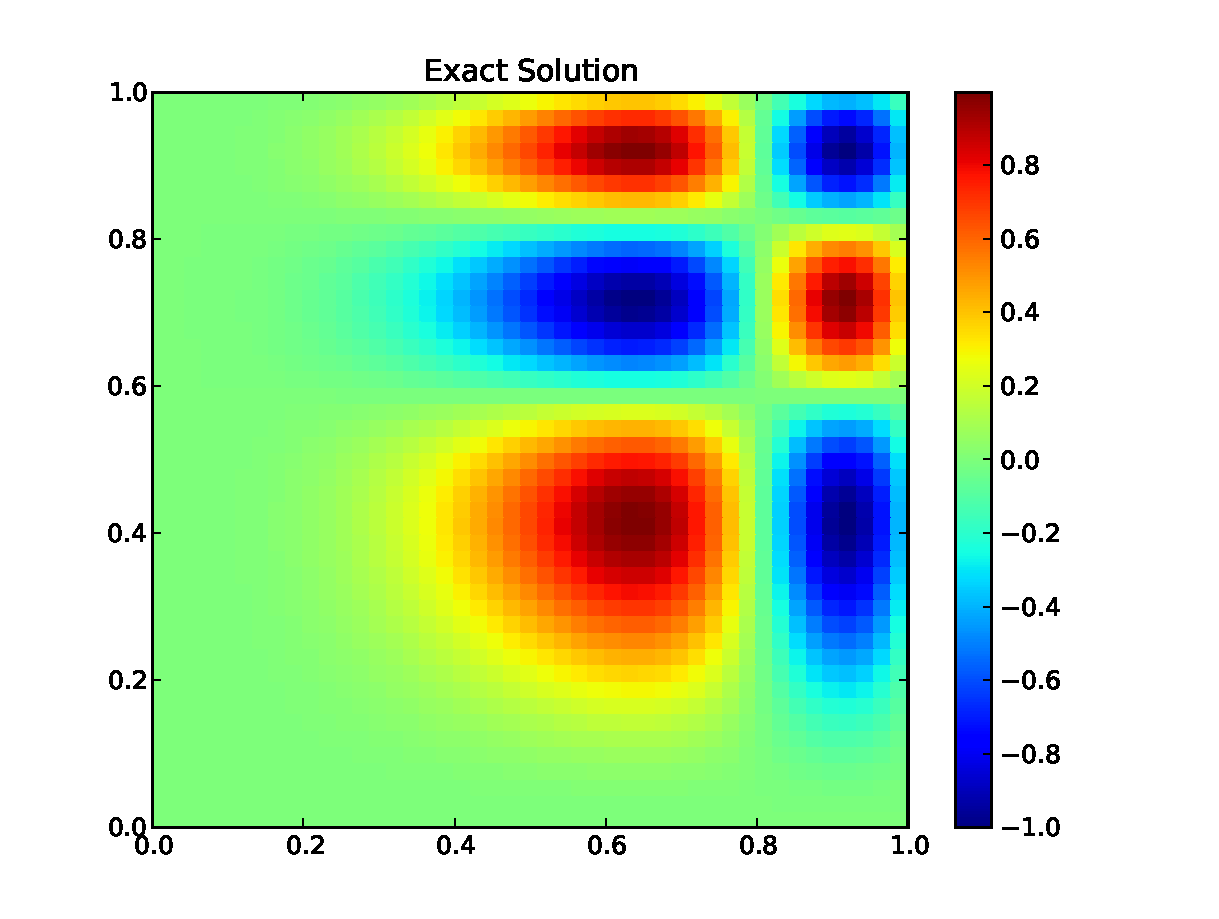
\includegraphics[width=5in,keepaspectratio]{Exact.pdf}
\end{center}
\caption{Exact solution}
\label{fig:Exact}
\end{figure}
\newpage 
\clearpage

\begin{figure}[h]
\begin{center}
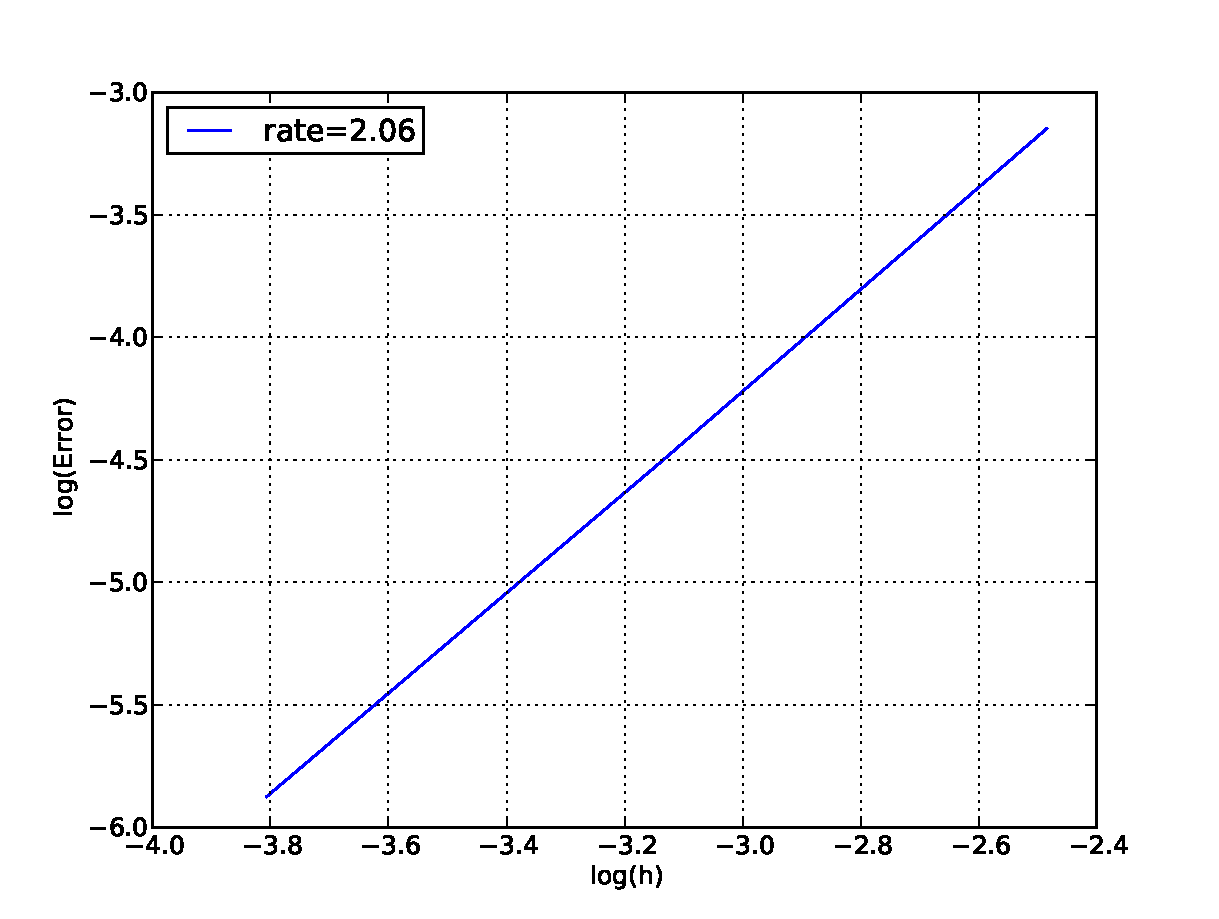
\includegraphics[width=4in,keepaspectratio]{c.pdf}
\end{center}
\caption{Second order finite difference convergence}
\label{fig:c}
\end{figure}
\lstinputlisting[language=Python,title={FDSolver.py}]{FDSolver.py}

\end{document}
